In the test cases, the energy management problem is formulated similarly to the formulation discussed in section \ref{formulation}. The  SOC of the ESS is discretized in steps of 2\% and the SOC is limited between  94\%  and  10\%. The time step chosen is 15 minutes. The ES is allowed to charge or discharge a maximum of 8\% of its total capacity during one time step. The 8\% limitation is set based on the specifications discussed in table \ref{tab:es}. The A* search is run every 15 minutes considering a prediction horizon of 24 hours (96 timesteps). The performances of the A* based ESM is tested for two different test scenarios. In scenario 1 the system is tested against a Sampling-Based Model Predictive Control (SBMPC) \colorbox{BurntOrange}{(CITE DOCTDER JOURNAL)}.In this case, net metering is assumed to maintain similarity with the other case. In scenario 2 the ESM is tested against two simple base test cases using both price data used in the first scenario and price data collected from PG\&E. In this scenario it is assumed buying and selling energy has different rates. In the testing phase the 

\subsection{Comparison with SBMPC and net metering}
Model predictive control (MPC) uses a predictive model to optimize a cost function while enforcing constraints on the system inputs and outputs and is widely applied in industrial process control \cite{qin1997overview}. Typically, industrial MPC is implemented for linear models, but the use of nonlinear models allows better performance over a wider operating range \cite{berber2012nonlinear}. SBMPC \cite{dunlap2011book}, \cite{reese2016graph} is an MPC method that uses a receding horizon along with the optimization algorithm, Sampling-Based Model Predictive Optimization (SBMPO), which samples the input of the predictive model to compute a  graph tree with nodes and branches. In \colorbox{BurntOrange}{(CITE DOCTDER JOURNAL)} the researchers use SBMPO to manage the energy at the PCC of a microgrid similar to the one described in section \ref{sys}. Figure \ref{fig:SBMPO_COMP_1_day} the 1 day test result for the A* based EMS considering the RTP scheme shown in Figure \ref{fig:RTP_PROFILE_8} and considering net metering. The price of the energy storage is calculated according to the specifications of Tesla Powerpack \cite{tesla_powerpack_2018}. The solid black line in the figure represents the SOC of the energy storage and the dotted red line represent the RTP. The left vertical axis of the figures represents the RTP of energy and the SOC of the ES. The right vertical axis represents the kWh demand of the system. A negative demand represents excess energy from the local generation after full filling the local demand. The bottom horizontal axis represents 15 minute time steps. The green arrows with the numbers represent specific parts of the figure used in the following explanation of the behavior of the EMS. As it can be seen in the figure that there are two peaks in price at the points 1 and 3 throughout the 24 hour (96 time step) window of operation.  The ESM properly anticipates the peak in point 1 and charges the energy storage using the grid just before the peak and discharges during the price peak at point 1. It can be seen that during the peak the demand was positive and the cheapest available price for grid energy was available just before the peak. The algorithm also anticipates the next peak based on forecasted data and prepares the ES to discharge at that peak by charging at the lowest RTP period at point 2. Although there is an excess generation available from the PV in between point 2 and point 3 the opportunity cost of using the PV to charge the ES will be equal to the RTP due to net metering. So, in this case, the algorithm behaves as expected and uses the lowest possible RTP period to charge the ES and discharges during the price period when there is a high enough price peak to justify the use of the energy storage.
 
  \begin{figure}[!ht]
    \centering
    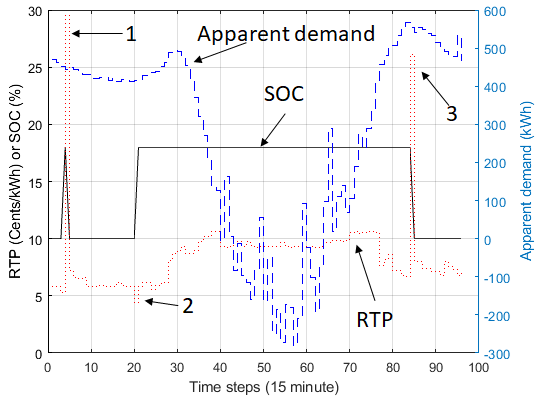
\includegraphics[width = \linewidth]{figs/SBMPO_COMP_1_day.png}
    \caption{EMS response for SBMPC comparison case}
    \label{fig:SBMPO_COMP_1_day}
\end{figure}

 Figure \ref{fig:SBMPO_COMP_10_12} shows the response of the A* based EMS for 7 days for the same system. The legend and axis notations used in the figure are similar to the one used in Figure \ref{fig:SBMPO_COMP_1_day}. It can be seen in the figure that the A* based ESM is following the behavior displayed in Figure \ref{fig:SBMPO_COMP_1_day}. It is taking advantage of the lowest price before a price peak and charging the energy storage in order to discharge the energy storage when there is a high enough price peak. The total cost of operation for the A* based ESM for the 7 day period is 4.8610e+03 \$. The SBMPO based scheme had a total cost of 4.9119e+03 \$ for the same 7 days. Compared to the results of the SBMPO based method described in \colorbox{BurntOrange}{(CITE DOCTDER JOURNAL)} the A* based method shows a savings of 1.04\% in the 7 day period.
 
 \begin{figure}[!ht]
    \centering
    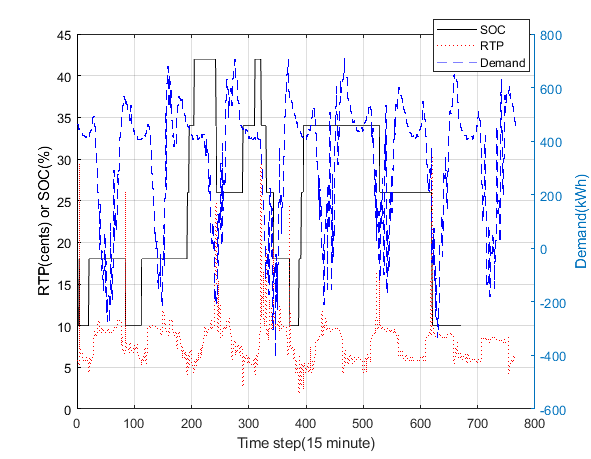
\includegraphics[width = \linewidth]{figs/SBMPO_COMP_10_12.png}
    \caption{EMS response for SBMPC comparison case}
    \label{fig:SBMPO_COMP_10_12}
\end{figure}


\subsection{Test result considering different buying and selling price}
In this scenario, the algorithm is tested against two base test cases using different price for selling power back to the grid. The different test cases:
\begin{enumerate}

\item \textbf{Case 1:} Charging from 2 AM to 5 AM, Discharging from 7 PM to 11 PM

\item \textbf{Case 2:} Charging from 11 AM to 2 PM, Discharging from 7 PM to 11 PM

\item \textbf{Case 3:}  A* based ESM control
\end{enumerate}

The cases 1 and 2 are standard control strategies based on predefined charging and discharging of the energy storage. Case 3 corresponds with A* based ESM control with a time step of 15 minutes and a prediction horizon of 24-hours. In these test cases, it is assumed the energy storage starts at the lower bound of SOC (10 \%).

Figure \ref{fig:VAR_1_day_example} shows the 1 day test result for the A* based EMS considering the RTP scheme shown in Figure \ref{fig:RTP_PROFILE_8} and considering a sell back price of 4 cents/kWh. The other system parameters are kept similar to the system used in the previous scenario. The legend and axis notations used in the figure are similar to the one used in Figure \ref{fig:SBMPO_COMP_1_day}. As it can be seen in the figure that there are two peaks in price at the points 1 and 3 throughout the 24 hour (96 time step) window of operation. The ESM properly anticipates the peak in point 1 and charges the energy storage using the grid just before the peak and discharges during the price peak at point 1 similar to the behavior observed in the previous scenario. The next price peak is at point 3 and the lowest price for grid power available for charging the storage is at point 4. In case of a net metering scheme, point 4 would have been the best time to charge the ES in order to discharge during the next price peak. Due to considering a sell back price of 4 cents/kWh this is no longer the case. 4 cents/kWh is lower than the price of buying grid energy at point 4. So the A* based EMS takes into account the lower opportunity cost of selling power back to the grid and decides to charge the ES during point 2 when there is extra local generation available. This behavior signifies that the A* based ESM can use the forecasted knowledge of the future demand and RTP together to decide the best moments to operate the energy storage depending on different pricing schemes.
 \begin{figure}[!ht]
    \centering
    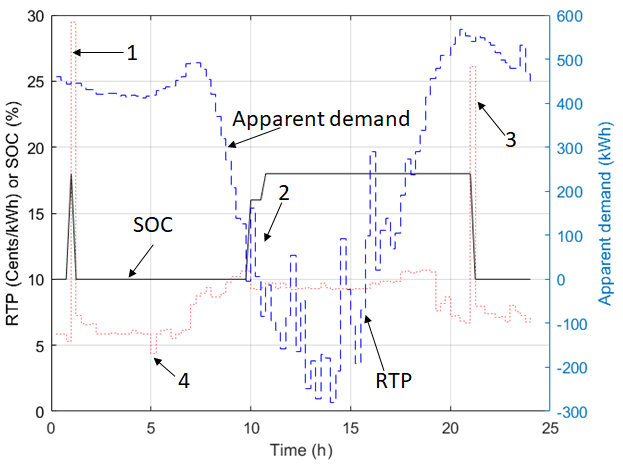
\includegraphics[width = \linewidth]{figs/VAR_1_day_example.png}
    \caption{1 day EMS response considering NYISO price and 4 centes/kWh sellback price}
    \label{fig:VAR_1_day_example}
\end{figure}

Figure \ref{fig:VAR_10_12_4} shows the 7 day test result for the microgrid considering the RTP shown in Figure \ref{fig:RTP_PROFILE_8} and a sell back price of 4 cents/kWh. Figure \ref{fig:VAR_10_12_30rtp} shows the 7 day test results for the same RTP considering a sell back price of 30\% of the RTP. Figure \ref{fig:PG_VAR_10_12_4} and Figure \ref{fig:PG_VAR_10_12_30rtp} shows the ESM operation for the PG\&E profile shown in Figure \ref{fig:PGNE_PRICE} considering 4 cents/kWh and 30\% of the RTP sell back price respectively. These figures follow the same legend and axis notations used in Figure \ref{fig:SBMPO_COMP_1_day}. It can be seen from the 7 day cases that the A* based ESM shows behavior similar to the behavior seen in  Figure \ref{fig:VAR_1_day_example}. The costs for the different conditions considered in the three cases are shown  Table \ref{tab:Cost}. The percentage cost comparison between the different cases is shown in Table \ref{tab:Cost_comp}. It can be seen from the table that depending on the test case the A* based ESM shows a cost savings of 6.93\% to 41.79\%. 
 \begin{figure}[!ht]
    \centering
    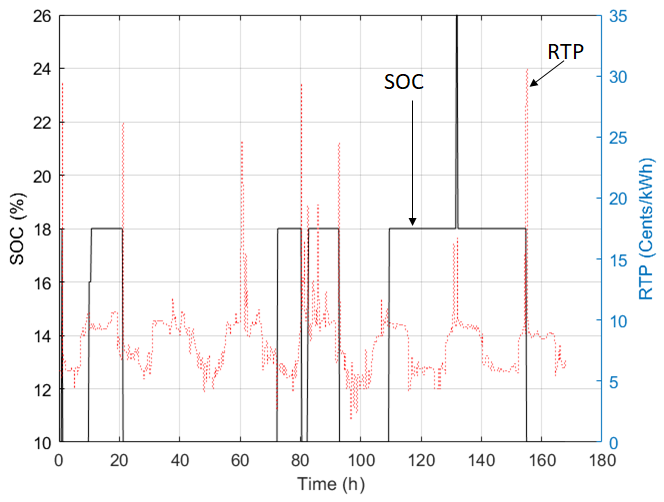
\includegraphics[width = \linewidth]{figs/VAR_10_12_4.png}
    \caption{7 day EMS response considering NYISO price and 4 centes/kWh sell back price}
    \label{fig:VAR_10_12_4}
\end{figure}

 \begin{figure}[!ht]
    \centering
    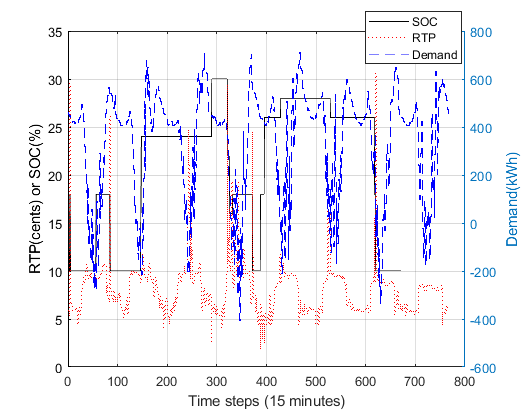
\includegraphics[width = \linewidth]{figs/VAR_10_12_30rtp.png}
    \caption{7 day EMS response considering NYISO price and 30\% of RTP sell back price}
    \label{fig:VAR_10_12_30rtp}
\end{figure}

 \begin{figure}[!ht]
    \centering
    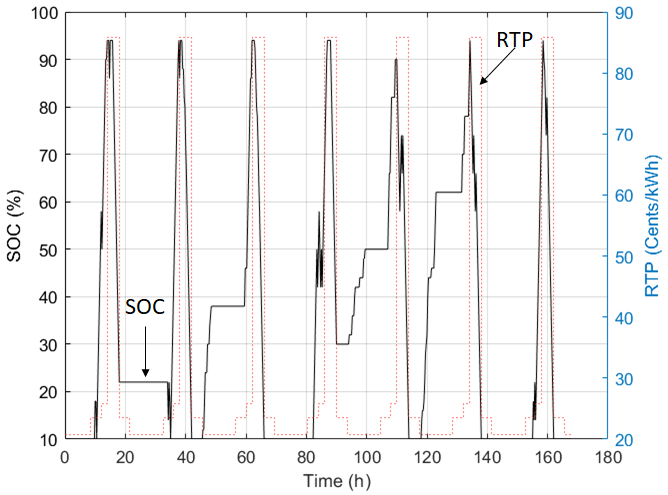
\includegraphics[width = \linewidth]{figs/PG_VAR_10_12_4.png}
    \caption{7 day EMS response considering PG\&E price and 4 centes/kWh sell back price}
    \label{fig:PG_VAR_10_12_4}
\end{figure}

 \begin{figure}[!ht]
    \centering
    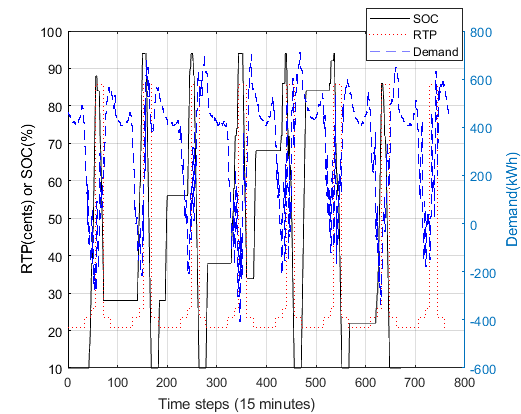
\includegraphics[width = \linewidth]{figs/PG_VAR_10_12_30rtp.png}
    \caption{7 day EMS response considering PG\&E price and 30\% of RTP sell back price}
    \label{fig:PG_VAR_10_12_30rtp}
\end{figure}


%%%%%%%%CSOT%%%%%%%%%%%%%%%%%%%%%%%%%%%%%%%%%%%
\begin{table}[htb]
\normalsize
\renewcommand{\arraystretch}{1}
\caption{Cost for the three cases}
\label{tab:Cost}
\centering
\resizebox{3.6in}{!}{%
\begin{tabular}{l|l|l|l|l|}
\cline{2-5}
                            & \multicolumn{2}{l|}{4 cents/kWh} & \multicolumn{2}{l|}{30\% RTP}   \\ \cline{2-5} 
                            & NYISO           & PG\&E          & NYISO          & PG\&E          \\ \hline
\multicolumn{1}{|l|}{Case1} & 8.2658e+03 \$  & 1.9396e+04 \$ & 8.3142e+03 \$ & 1.9109e+04 \$ \\ \hline
\multicolumn{1}{|l|}{Case2} & 8.8606e+03 \$  & 1.9633e+04 \$ & 8.8955e+03 \$ & 1.9407e+04 \$ \\ \hline
\multicolumn{1}{|l|}{Case3} & 5.3295e+03 \$  & 1.8051e+04 \$ & 5.1783e+03 \$ & 1.7106e+04 \$ \\ \hline
\multicolumn{1}{|l|}{Case3} & 5.3295e+03 \$  & 1.8051e+04 \$ & 5.1783e+03 \$ & 1.7106e+04 \$ \\ \hline
\end{tabular}
}
\end{table}
%%%%%%%%CSOT%%%%%%%%%%%%%%%%%%%%%%%%%%%%%%%%%%%




%%%%%%%%COMPARE_COST%%%%%%%%%%%%%%%%%%%%%%%%%%%%%%%%%%%
\begin{table}[htb]
\normalsize
\renewcommand{\arraystretch}{1}
\caption{Case 3 savings compared to other cases}
\label{tab:Cost_comp}
\centering
\begin{tabular}{l|l|l|l|l|}
\cline{2-5}
                            & \multicolumn{2}{l|}{4 cents/kWh} & \multicolumn{2}{l|}{30\% RTP}   \\ \cline{2-5} 
                            & NYISO           & PG\&E          & NYISO          & PG\&E          \\ \hline
\multicolumn{1}{|l|}{Case1} & 35.52\%         & 6.93\%         & 37.72\%        & 10.84\%        \\ \hline
\multicolumn{1}{|l|}{Case2} & 39.85\%         & 8.08\%         & 41.79\%        & 11.86\%        \\ \hline
\end{tabular}
\end{table}
%%%%%%%%COMPARE_COST%%%%%%%%%%%%%%%%%%%%%%%%%%%%%%%%%%%